\section{Relation between physically based parameters and BSSRDF parametrization}
\label{section:cb_parametrization}
The Monte Carlo methods of light simulation based on the radiative transport equation use
$\sigma_a$, $\sigma_s$ and $phase function$ as a set parameters defining the optical properties of
the SSS materials \cite{chandrasekhar1960radiative}, \cite{pharr2010physically},
\cite{Jensen:2001:PMS:383259.383319}.

This chapter covers only the case of isotropic media. That is why the phase function is assumed to
be constant. The short overview of an anisotropic media and complex phase function approximations
can be found in the sections \ref{section:phasefunction} and \ref{section:ptdl_implement}.

In contrast to the Monte Carlo methods, BSSRDF profiles for the Diffusion approximation, relay on
the surface albedo (diffuse surface reflectance) parameter $A$ of the material:
\[ A = \int\limits_0^\infty R(r)2\pi r dr \]

Which has the meaning of the integral amount of the outgoing radiant exitance over the whole area of
the object relative to the overall incoming irradiance. In order to maintain consistent
parametrization for different SSS integration techniques, the physically based parameters $\sigma_a$
and $\sigma_s$ have to be mapped to the surface albedo $A$ used by Diffusion Approximation.

As an intermediate representation of the physically based parameters I use volumetric scattering
albedo: $\alpha = \sigma_s/\sigma_t = \sigma_s/(\sigma_s + \sigma_a)$. This parametrization is
commonly used in diffusion approximation \cite{Jensen:2002:RHR:566570.566619},
\cite{Donner:2009:EBM}.

In the classic work on this topic \emph{'A Practical Model for Subsurface Light Transport'} in the
section 2.4 \cite{Jensen:2001:PMS:383259.383319} proposed the analytic method of computing the
surface albedo $A$ out of the volumetric scattering albedo $\alpha$ with the assumption of the
incident uniform illumination.

This analytic approach accounts for the media with different \gls{IOR} by computing the
\emph{average diffuse Fresnel reflectance} and using reduced scattering coefficients to approximate
anisotropic media. The plot of the proposed function for the case of $IoR=1$ and $g=0$ is shown at
figure \ref{fig:albedo_fitting_techniques}.

\begin{figure}
    \centering
    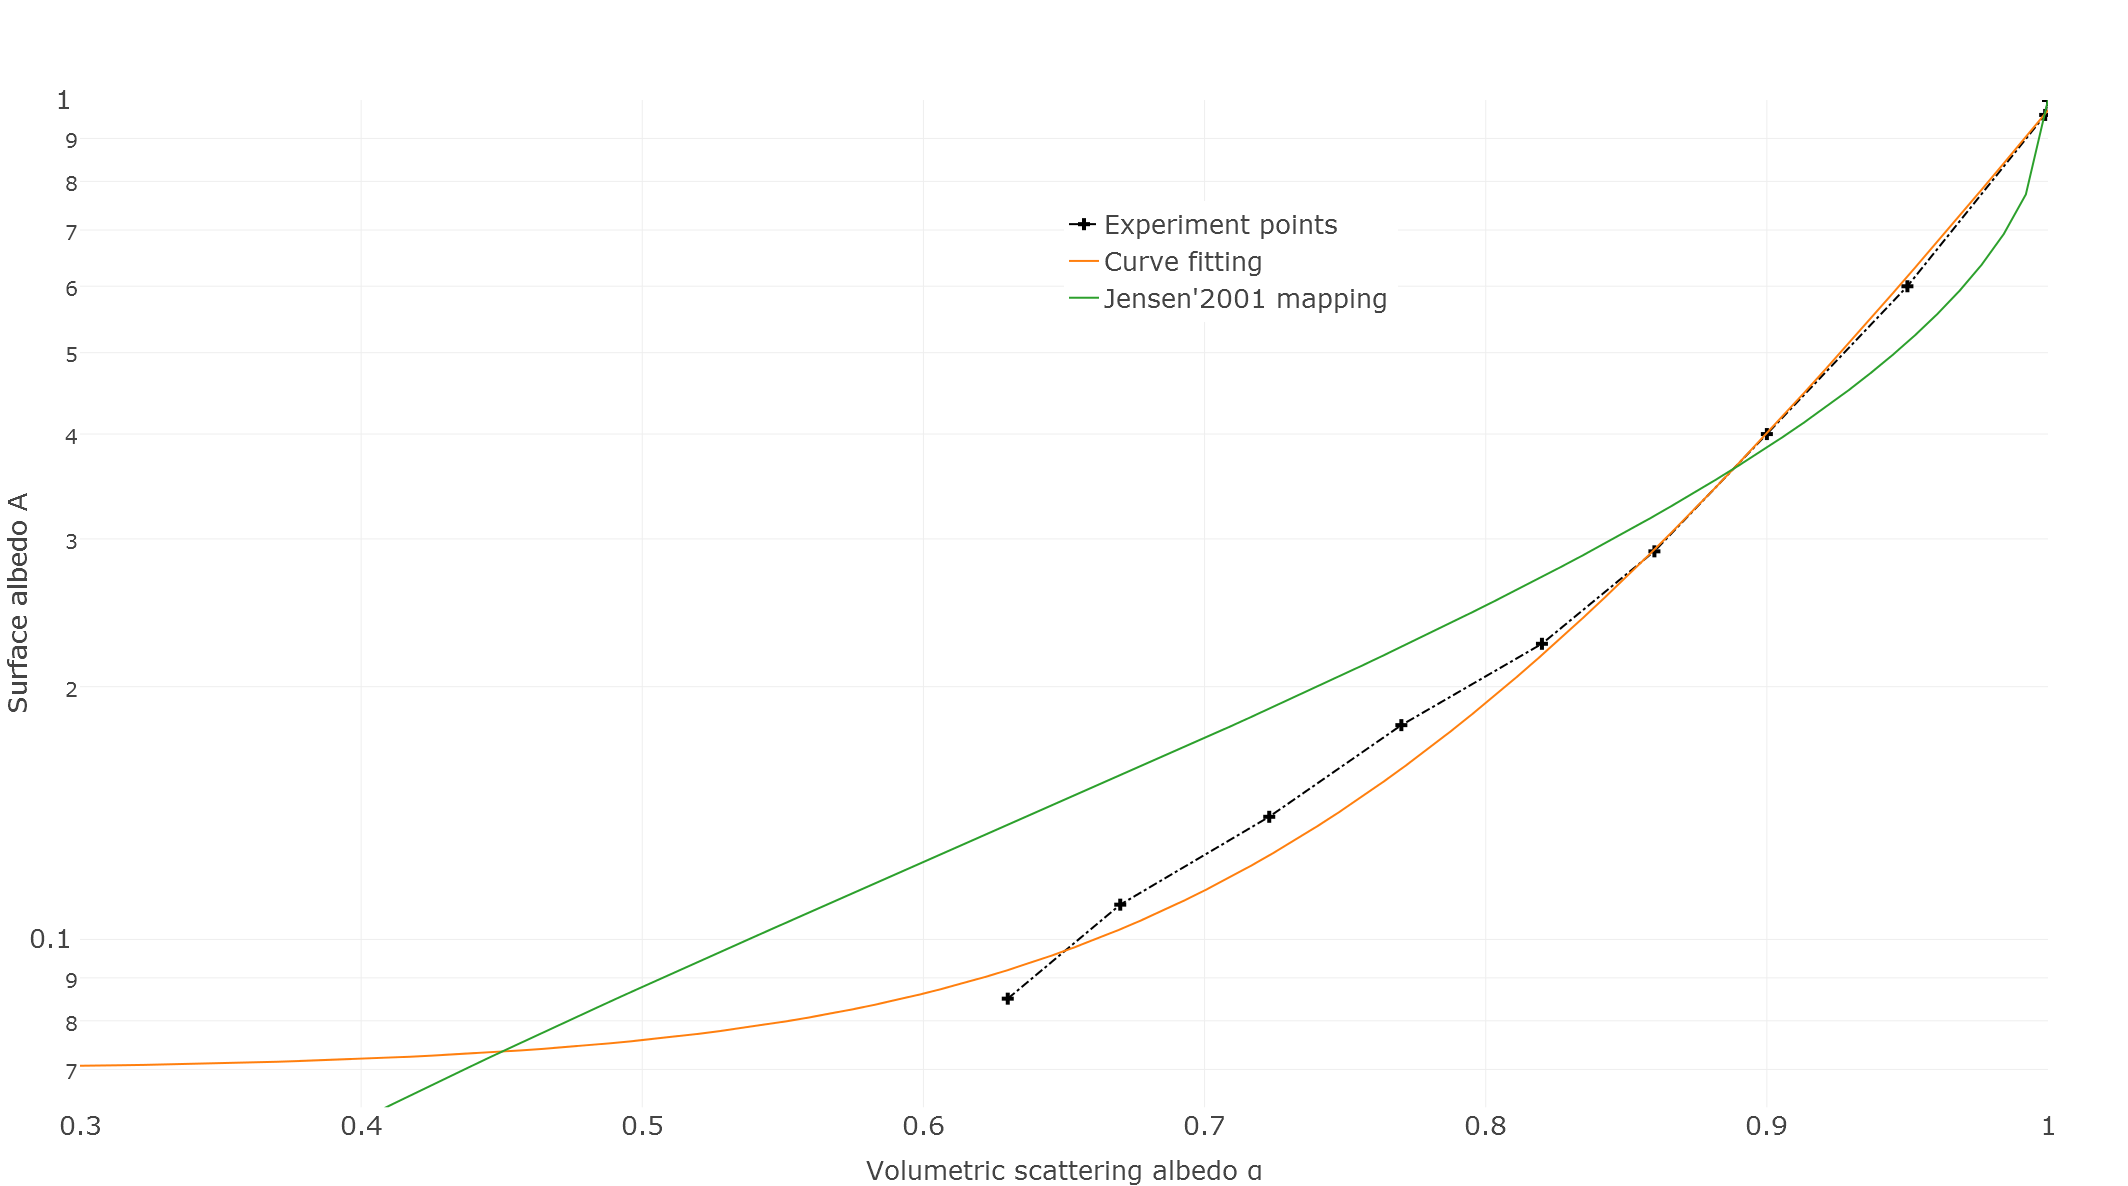
\includegraphics[width=0.98\textwidth]{imgs/plots/aA_fitting_methods}
    \caption{Comparison of the albedo mapping technique described in
    \cite{Jensen:2001:PMS:383259.383319} to the empirical curve fitting}
    \label{fig:albedo_fitting_techniques}
\end{figure}

In this work I propose the empirical approach to tackle this problem and find a good mapping with
the above mentioned assumption of isotropic media. The following function is proved to be a good fit
when rendering different materials:
\begin{equation}
\label{eq:aAMapping}
A(\alpha) = a + b(1- e^{-c\alpha})
\end{equation}
with corresponding constants: $a = 0.0699, b = -3.97\cdot 10^{-05}, c =-10.0$

The empirical mapping \ref{eq:aAMapping} shows better match \ref{fig:albedo_fitting_techniques} to
Christensen-Burley BSSRDF profiles to Monte Carlo references than analytic approach described by
\cite{Jensen:2001:PMS:383259.383319}.

The disadvantage of simpler empirical function is that in contrast to analytic approach it does not
account for Index of Refraction of the media and assume the isotropic media. The latter, however, is
already assumed by application of the Diffusion approximation.

\begin{figure}
    \centering
    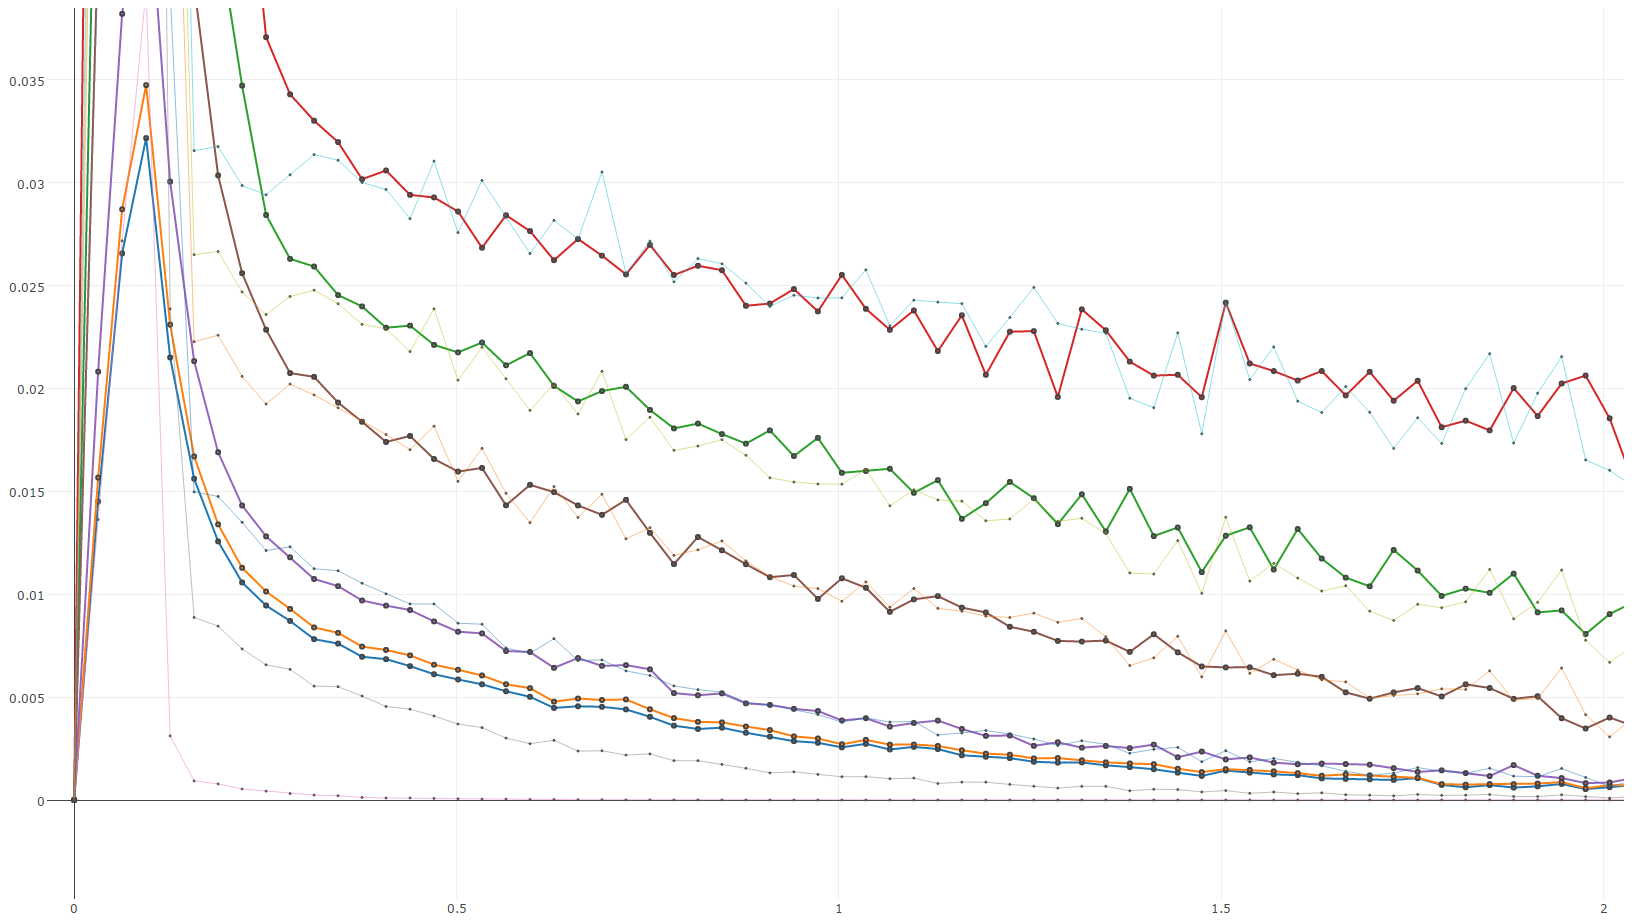
\includegraphics[width=0.98\textwidth]{imgs/plots/aA_fitting}
    \caption{Christensen-Burley BSSRDF profiles for materials with different albedo values. The
    curve fitting \ref{eq:aAMapping} was used to compute $A$ out of $\alpha$}
    \label{fig:albedo_fitting}
\end{figure}

The results of the fitting \ref{eq:aAMapping} are available at figure \ref{fig:albedo_fitting}. The
set of Monte Carlo reference curves are plotted in dashed lines. The corresponding BSSRDF curves
plotted in solid color using the surface albedo computed with the above mentioned fitting function.

As it is seen from the plots, the best fit is achieved for the materials with high volumetric
albedo approximately $\alpha\geq0.67$. But two lowest pairs of curves (green and red with
$\alpha=0.5$ and $\alpha=0.33$ respectively) demonstrate poor match.

This result is consistent with the assumptions of the diffusion theory of
the light transport in participating media. The good approximation can be done only for the high
albedo media without significant attenuation.